\subsection{Kort intruduktion till programmering i \coq och
Utvecklingsmiljön \coqIde}


\subsubsection{Interaktiv beskrivning av \coqIde}


\begin{figure}[h!]
  \centering
  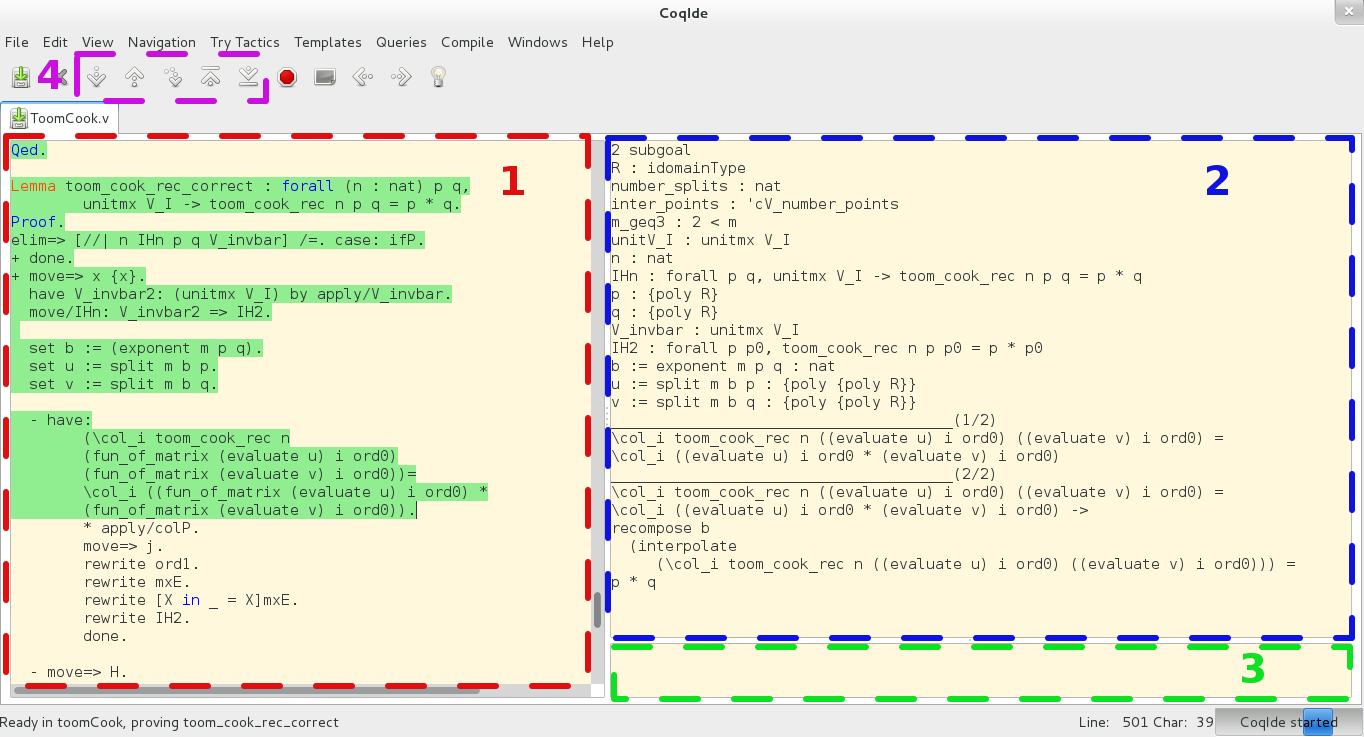
\includegraphics[width=150mm]{../images/Overview}
  \caption[Översikt av \coqIde]
   {Översikt av de olika delarna i \coqIde}
\end{figure}


\begin{enumerate}
\item Textredigerare. I den här rutan skriver användaren sina program och bevis
\item Textfönster för mål och kontext. Här visas vilka mål man vill uppnå och
  vilka värden man för närvarande har i kontext. Dessa uppdateras efter varje
  utförd taktik.
\item Textfönter för medelanden. Här dyker felmedelanden, svar på
  gjorda sökningar och övrig information.
\item Symboler för att stega framåt eller bakåt i koden. När vi stegar framåt
  så evalueras koden som stegas förbi.


\begin{figure}[h!]
  \centering
  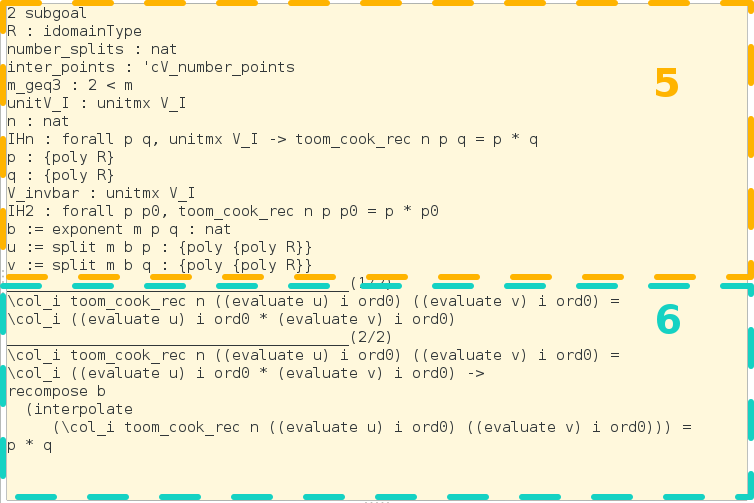
\includegraphics[width=150mm]{../images/Kontext}
  \caption[Fönster för kontext och mål]
   {Textfönster för kontext och mål. Detta är en försoring av (2) från
     föregående figur}
\end{figure}

Förstoring av (2)
\item Kontext, här visas vilka hypoteser och variabler som vi för tillfället
  har i beviset.
\item Mål, här visas vilka mål som ska uppnås. Det översta målet är det som
  användaren arbetar med för tillfället och det är det målet som kommer att
  påverkas av nästkommande taktik.
\end{enumerate}


\subsubsection{Evaluering av kod}
\coq är uppbygt av satser där varje sats avslutas med en punkt.
Koden evaluers sedan en sats i taget och de delar av koden som
har blivit evaluerade markeras med en grön färg och det går inte längre
att göra några ändringar i dessa. Om man skulle vilja göra en ändring så
får man i så fall stega tillbaks i programet och göra ändringen.

\subsubsection{Bevis}
Det finns flera olika nyckelord för att starta ett bevis bland annat
\C{theorem} och \C{lemma}. Det är ingen skillnad på vilket
av dessa orden man använder för att påbörja ett bevis utan de är bara
till för att användaren ska kunna gradera sina bevis. För enkelhetens skull
kommer bara nyckelordet \C{lemma} användas i fortsättningen. Ett bevis i
\coq är uppbyggt på följande sätt

\begin{lstlisting}
lemma bevisnamn : påstående som ska bevisas.
Proof.
  taktiker.
Qed.
\begin{lstlisting}

Här är ett exempel på ett bevis för att följande påstående är en tautalogi.

\begin{figure}[H]
  \centering
  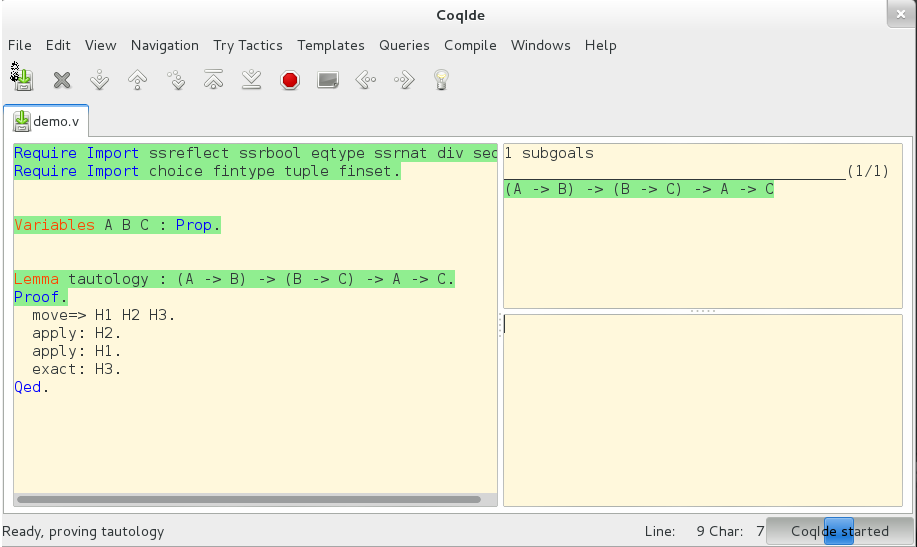
\includegraphics[width=100mm]{../images/Proof_part1}
  \caption[Exempel på bevis i \coq]
   {Exempel på ett bevis för en tautalogi i \coq}
\end{figure}


Om vi nu stegar igenom beviset så kan vi se att både målet och kontexten
förändras efter varje steg

\begin{figure}[H]
  \centering
  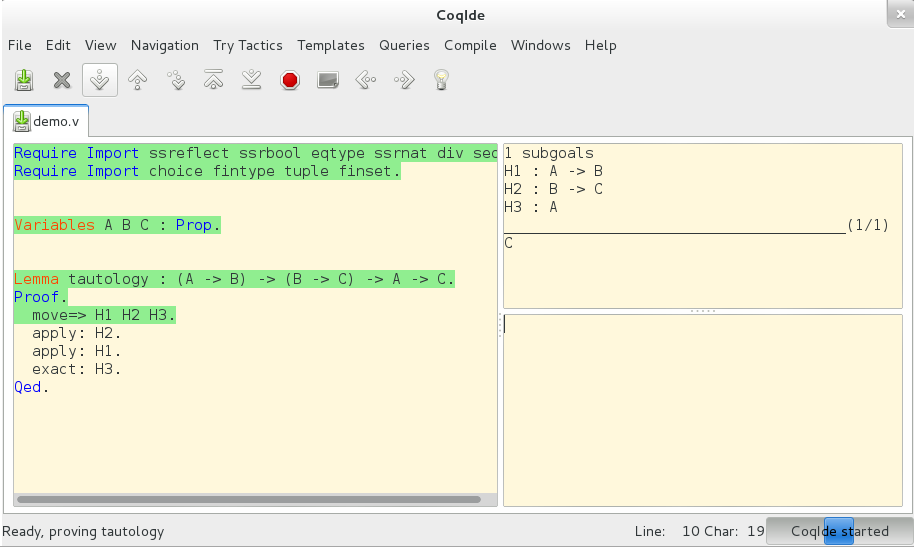
\includegraphics[width=150mm]{../images/Proof_part2}
  \caption[Bevis i \coqIde]
   {Vi har nu flyttat hypoteserna A medför B, B medför C och A
    från målet till kontexten och med taktiken move}
\end{figure}

\begin{figure}[H]
  \centering
  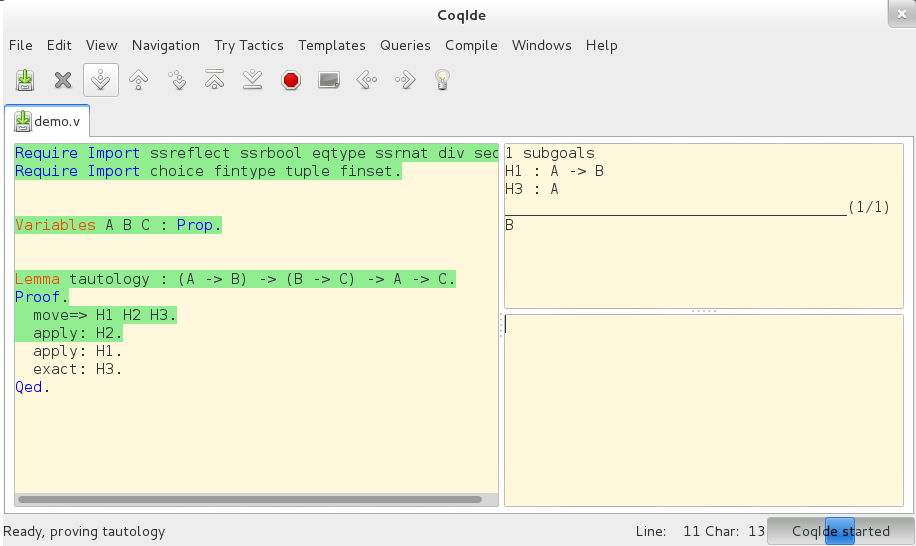
\includegraphics[width=150mm]{../images/Proof_part3}
  \caption[Bevis i \coqIde]
   {Vi har nu använt oss av Hypotesen B medför C och vi
    kan se att målet nu har ändrat sig från A till B}
\end{figure}


När alla mål är bevisade så talar man om att beviset är klart genom att
skriva  \C{Qed.} vilket översatt till svenska betyder
"Vilket skulle bevisas"


\subsection{Varibler och Funktioner}

Det går att definera varibler i \coq med nyckelordet \C{Varible}
När en variabel deklareras på global nivå kan den sedan användas som
parameter i bevis och funktionsdefinitioner utan att behöva ange typen.
En variabel kan också ses som en hypotes men mer om detta i stycket om
Curry Howard isomorphism


För att definera funktioner och konstanter så används nyckelordet
\C{Definition} som sedan sedan följs av funktions namn,
parametrar och funktionskropp.

\coq tillåter bara rekursion som är garanterad att terminera. Det vill
säga att någon av parametrarna i det rekursiva kallet måste närma sig
basfallet eller så måste användaren ange ett bevis för att funktionen är
garanterad att terminera. Så istället för att använda \C{Define}
för att definera en funktion så måste man använda \C{Fixpoint} istället.
Det skulle till exempel inte gå att göra en rekursiv
funktion för Collatz problem i \coq. Detta eftersom parametern bara minskar
om talet är jämt och det inte går att bevisa att basfallet alltid nås.

Collatz problem.
\begin{equation}
T(n) = \left\{\begin{matrix} n/2, & \mbox{om }n\equiv0\mbox{ (mod 2)} \\ 3n+1,
                         & \mbox{om }n\equiv1\mbox{ (mod 2)} \end{matrix}\right.
\end{equation}


\subsection{Patternmatching}

Patternmatchning i \coq påminner till stor del om \C{case} i Haskell.
Skilnaden är att istället för att skriva \C{case x of} som i Haskell
så skrivs \C{match x with} där x är namnet på variabeln ska matchas i
båda fallen. I \coq så måste även alla efterföljande rader utan den första
börja med symbolen $|$. Matchningssatsen måste även avslutas med \C{end}.

\begin{figure}[H]
  \centering
  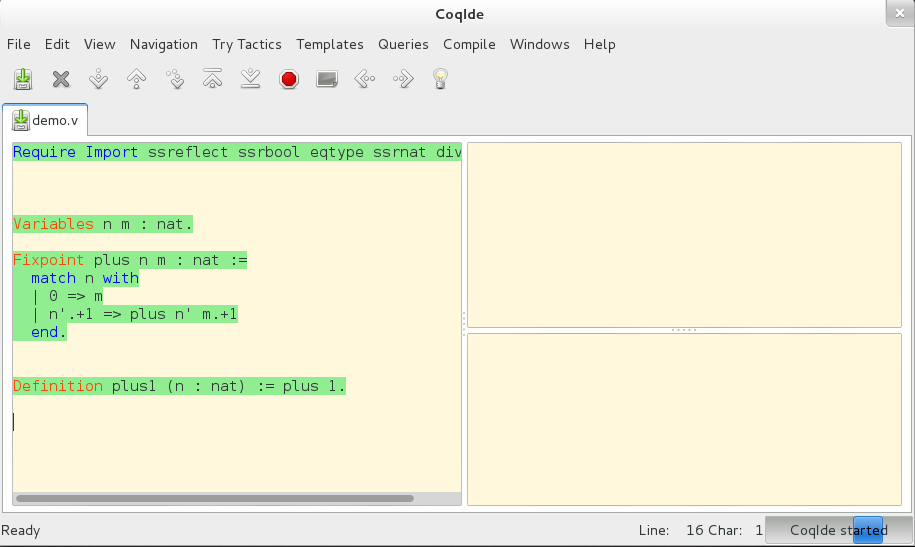
\includegraphics[width=150mm]{../images/Variables_and_Functions}
  \caption[Variabler och funktioner]
   {Exempel på hur variabler och funktioner defineras i \coq}
\end{figure}